\documentclass{standalone}
\usepackage{tikz}
\usetikzlibrary{patterns, positioning}


\begin{document}
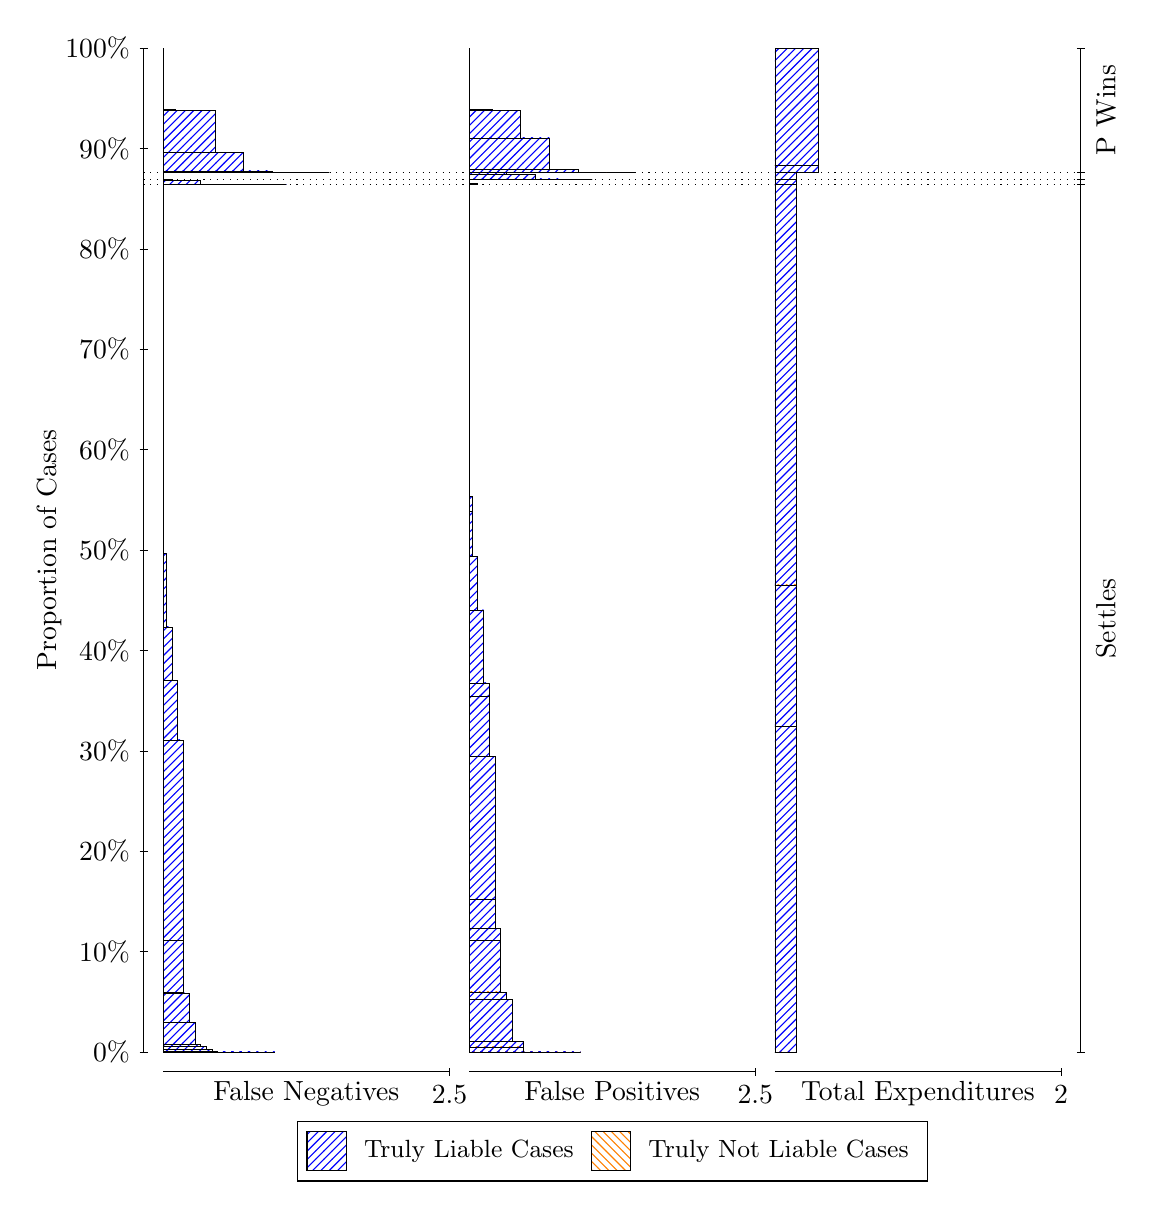
\begin{tikzpicture}
\draw[black, very thin] (1.5,1.75) -- (1.5,14.5);
\node[rotate=90, text=black, anchor=center] at (0.3, 8.125) {Proportion of Cases};
\draw[black, very thin] (1.45,1.75) -- (1.55,1.75);
\node[text=black, anchor=east] at (1.45, 1.75) {0\%};
\draw[black, very thin] (1.45,3.025) -- (1.55,3.025);
\node[text=black, anchor=east] at (1.45, 3.025) {10\%};
\draw[black, very thin] (1.45,4.3) -- (1.55,4.3);
\node[text=black, anchor=east] at (1.45, 4.3) {20\%};
\draw[black, very thin] (1.45,5.575) -- (1.55,5.575);
\node[text=black, anchor=east] at (1.45, 5.575) {30\%};
\draw[black, very thin] (1.45,6.85) -- (1.55,6.85);
\node[text=black, anchor=east] at (1.45, 6.85) {40\%};
\draw[black, very thin] (1.45,8.125) -- (1.55,8.125);
\node[text=black, anchor=east] at (1.45, 8.125) {50\%};
\draw[black, very thin] (1.45,9.4) -- (1.55,9.4);
\node[text=black, anchor=east] at (1.45, 9.4) {60\%};
\draw[black, very thin] (1.45,10.675) -- (1.55,10.675);
\node[text=black, anchor=east] at (1.45, 10.675) {70\%};
\draw[black, very thin] (1.45,11.95) -- (1.55,11.95);
\node[text=black, anchor=east] at (1.45, 11.95) {80\%};
\draw[black, very thin] (1.45,13.225) -- (1.55,13.225);
\node[text=black, anchor=east] at (1.45, 13.225) {90\%};
\draw[black, very thin] (1.45,14.5) -- (1.55,14.5);
\node[text=black, anchor=east] at (1.45, 14.5) {100\%};

\draw[black, very thin] (13.4,1.75) -- (13.4,14.5);
\draw[black, very thin] (13.35,1.75) -- (13.45,1.75);
\node[anchor=west] at (13.35, 1.75) {};
\draw[black, very thin] (13.35,12.765) -- (13.45,12.765);
\node[anchor=west] at (13.35, 12.765) {};
\draw[black, very thin] (13.35,12.834) -- (13.45,12.834);
\node[anchor=west] at (13.35, 12.834) {};
\draw[black, very thin] (13.35,12.923) -- (13.45,12.923);
\node[anchor=west] at (13.35, 12.923) {};
\draw[black, very thin] (13.35,14.5) -- (13.45,14.5);
\node[anchor=west] at (13.35, 14.5) {};

\draw[black, very thin, pattern color=blue, pattern=north east lines] (1.75,1.75) rectangle (3.167,1.75);
\draw[black, very thin, pattern color=blue, pattern=north east lines] (1.75,1.75) rectangle (3.0217,1.75);
\draw[black, very thin, pattern color=blue, pattern=north east lines] (1.75,1.75) rectangle (2.8763,1.75);
\draw[black, very thin, pattern color=blue, pattern=north east lines] (1.75,1.75) rectangle (2.8037,1.75);
\draw[black, very thin, pattern color=blue, pattern=north east lines] (1.75,1.75) rectangle (2.731,1.75);
\draw[black, very thin, pattern color=blue, pattern=north east lines] (1.75,1.75) rectangle (2.6583,1.75);
\draw[black, very thin, pattern color=blue, pattern=north east lines] (1.75,1.75) rectangle (2.5857,1.75);
\draw[black, very thin, pattern color=blue, pattern=north east lines] (1.75,1.75) rectangle (2.513,1.7518);
\draw[black, very thin, pattern color=blue, pattern=north east lines] (1.75,1.7518) rectangle (2.4403,1.7592);
\draw[black, very thin, pattern color=blue, pattern=north east lines] (1.75,1.7592) rectangle (2.3677,1.7592);
\draw[black, very thin, pattern color=blue, pattern=north east lines] (1.75,1.7592) rectangle (2.3677,1.7871);
\draw[black, very thin, pattern color=blue, pattern=north east lines] (1.75,1.7871) rectangle (2.295,1.8177);
\draw[black, very thin, pattern color=blue, pattern=north east lines] (1.75,1.8177) rectangle (2.2223,1.8509);
\draw[black, very thin, pattern color=blue, pattern=north east lines] (1.75,1.8509) rectangle (2.1497,2.1291);
\draw[black, very thin, pattern color=blue, pattern=north east lines] (1.75,2.1291) rectangle (2.1497,2.1291);
\draw[black, very thin, pattern color=blue, pattern=north east lines] (1.75,2.1291) rectangle (2.077,2.5012);
\draw[black, very thin, pattern color=blue, pattern=north east lines] (1.75,2.5012) rectangle (2.0043,2.5025);
\draw[black, very thin, pattern color=blue, pattern=north east lines] (1.75,2.5025) rectangle (2.0043,3.1706);
\draw[black, very thin, pattern color=blue, pattern=north east lines] (1.75,3.1706) rectangle (2.0043,5.7124);
\draw[black, very thin, pattern color=blue, pattern=north east lines] (1.75,5.7124) rectangle (1.9317,6.4669);
\draw[black, very thin, pattern color=blue, pattern=north east lines] (1.75,6.4669) rectangle (1.859,7.1496);
\draw[black, very thin, pattern color=blue, pattern=north east lines] (1.75,7.1496) rectangle (1.7863,8.0776);
\draw[black, very thin, pattern color=blue, pattern=north east lines] (1.75,8.0776) rectangle (1.7863,8.0776);
\draw[black, very thin, pattern color=orange, pattern=north west lines] (1.75,8.0776) rectangle (1.75,8.0776);
\draw[black, very thin, pattern color=blue, pattern=north east lines] (1.75,8.0776) rectangle (1.75,12.765);
\draw[black, very thin, pattern color=blue, pattern=north east lines] (1.75,12.765) rectangle (3.3123,12.765);
\draw[black, very thin, pattern color=blue, pattern=north east lines] (1.75,12.765) rectangle (2.949,12.765);
\draw[black, very thin, pattern color=blue, pattern=north east lines] (1.75,12.765) rectangle (2.5857,12.769);
\draw[black, very thin, pattern color=blue, pattern=north east lines] (1.75,12.769) rectangle (2.2223,12.816);
\draw[black, very thin, pattern color=blue, pattern=north east lines] (1.75,12.816) rectangle (1.859,12.834);
\draw[black, very thin, pattern color=orange, pattern=north west lines] (1.75,12.834) rectangle (1.75,12.834);
\draw[black, very thin, pattern color=blue, pattern=north east lines] (1.75,12.834) rectangle (1.859,12.835);
\draw[black, very thin, pattern color=orange, pattern=north west lines] (1.75,12.835) rectangle (1.75,12.835);
\draw[black, very thin, pattern color=blue, pattern=north east lines] (1.75,12.835) rectangle (1.75,12.923);
\draw[black, very thin, pattern color=blue, pattern=north east lines] (1.75,12.923) rectangle (3.8573,12.923);
\draw[black, very thin, pattern color=blue, pattern=north east lines] (1.75,12.923) rectangle (3.494,12.923);
\draw[black, very thin, pattern color=blue, pattern=north east lines] (1.75,12.923) rectangle (3.1307,12.94);
\draw[black, very thin, pattern color=blue, pattern=north east lines] (1.75,12.94) rectangle (2.7673,13.177);
\draw[black, very thin, pattern color=blue, pattern=north east lines] (1.75,13.177) rectangle (2.622,13.177);
\draw[black, very thin, pattern color=blue, pattern=north east lines] (1.75,13.177) rectangle (2.404,13.704);
\draw[black, very thin, pattern color=blue, pattern=north east lines] (1.75,13.704) rectangle (2.2587,13.704);
\draw[black, very thin, pattern color=blue, pattern=north east lines] (1.75,13.704) rectangle (2.0407,13.705);
\draw[black, very thin, pattern color=blue, pattern=north east lines] (1.75,13.705) rectangle (1.8953,13.716);
\draw[black, very thin, pattern color=orange, pattern=north west lines] (1.75,13.716) rectangle (1.75,13.716);
\draw[black, very thin, pattern color=blue, pattern=north east lines] (1.75,13.716) rectangle (1.75,14.5);
\draw[black, very thin, pattern color=orange, pattern=north west lines] (5.6333,1.75) rectangle (7.0503,1.75);
\draw[black, very thin, pattern color=blue, pattern=north east lines] (5.6333,1.75) rectangle (7.0503,1.75);
\draw[black, very thin, pattern color=orange, pattern=north west lines] (5.6333,1.75) rectangle (6.905,1.75);
\draw[black, very thin, pattern color=blue, pattern=north east lines] (5.6333,1.75) rectangle (6.905,1.75);
\draw[black, very thin, pattern color=orange, pattern=north west lines] (5.6333,1.75) rectangle (6.7597,1.75);
\draw[black, very thin, pattern color=blue, pattern=north east lines] (5.6333,1.75) rectangle (6.7597,1.75);
\draw[black, very thin, pattern color=blue, pattern=north east lines] (5.6333,1.75) rectangle (6.687,1.75);
\draw[black, very thin, pattern color=orange, pattern=north west lines] (5.6333,1.75) rectangle (6.6143,1.75);
\draw[black, very thin, pattern color=blue, pattern=north east lines] (5.6333,1.75) rectangle (6.6143,1.75);
\draw[black, very thin, pattern color=blue, pattern=north east lines] (5.6333,1.75) rectangle (6.5417,1.7501);
\draw[black, very thin, pattern color=orange, pattern=north west lines] (5.6333,1.7501) rectangle (6.469,1.7501);
\draw[black, very thin, pattern color=blue, pattern=north east lines] (5.6333,1.7501) rectangle (6.469,1.751);
\draw[black, very thin, pattern color=blue, pattern=north east lines] (5.6333,1.751) rectangle (6.3963,1.7517);
\draw[black, very thin, pattern color=orange, pattern=north west lines] (5.6333,1.7517) rectangle (6.3237,1.7517);
\draw[black, very thin, pattern color=blue, pattern=north east lines] (5.6333,1.7517) rectangle (6.3237,1.8133);
\draw[black, very thin, pattern color=orange, pattern=north west lines] (5.6333,1.8133) rectangle (6.3237,1.8133);
\draw[black, very thin, pattern color=blue, pattern=north east lines] (5.6333,1.8133) rectangle (6.3237,1.8801);
\draw[black, very thin, pattern color=blue, pattern=north east lines] (5.6333,1.8801) rectangle (6.251,1.8831);
\draw[black, very thin, pattern color=orange, pattern=north west lines] (5.6333,1.8831) rectangle (6.1783,1.8831);
\draw[black, very thin, pattern color=blue, pattern=north east lines] (5.6333,1.8831) rectangle (6.1783,2.4143);
\draw[black, very thin, pattern color=blue, pattern=north east lines] (5.6333,2.4143) rectangle (6.1057,2.5122);
\draw[black, very thin, pattern color=orange, pattern=north west lines] (5.6333,2.5122) rectangle (6.033,2.5122);
\draw[black, very thin, pattern color=blue, pattern=north east lines] (5.6333,2.5122) rectangle (6.033,3.1669);
\draw[black, very thin, pattern color=blue, pattern=north east lines] (5.6333,3.1669) rectangle (6.033,3.3202);
\draw[black, very thin, pattern color=blue, pattern=north east lines] (5.6333,3.3202) rectangle (5.9603,3.6944);
\draw[black, very thin, pattern color=blue, pattern=north east lines] (5.6333,3.6944) rectangle (5.9603,5.5029);
\draw[black, very thin, pattern color=orange, pattern=north west lines] (5.6333,5.5029) rectangle (5.8877,5.5029);
\draw[black, very thin, pattern color=blue, pattern=north east lines] (5.6333,5.5029) rectangle (5.8877,6.2716);
\draw[black, very thin, pattern color=blue, pattern=north east lines] (5.6333,6.2716) rectangle (5.8877,6.4372);
\draw[black, very thin, pattern color=blue, pattern=north east lines] (5.6333,6.4372) rectangle (5.815,7.3652);
\draw[black, very thin, pattern color=blue, pattern=north east lines] (5.6333,7.3652) rectangle (5.7423,8.0479);
\draw[black, very thin, pattern color=blue, pattern=north east lines] (5.6333,8.0479) rectangle (5.6697,8.6228);
\draw[black, very thin, pattern color=blue, pattern=north east lines] (5.6333,8.6228) rectangle (5.6697,8.8024);
\draw[black, very thin, pattern color=blue, pattern=north east lines] (5.6333,8.8024) rectangle (5.6333,12.765);
\draw[black, very thin, pattern color=orange, pattern=north west lines] (5.6333,12.765) rectangle (5.7423,12.765);
\draw[black, very thin, pattern color=blue, pattern=north east lines] (5.6333,12.765) rectangle (5.7423,12.783);
\draw[black, very thin, pattern color=blue, pattern=north east lines] (5.6333,12.783) rectangle (5.6333,12.834);
\draw[black, very thin, pattern color=orange, pattern=north west lines] (5.6333,12.834) rectangle (7.1957,12.834);
\draw[black, very thin, pattern color=blue, pattern=north east lines] (5.6333,12.834) rectangle (7.1957,12.834);
\draw[black, very thin, pattern color=blue, pattern=north east lines] (5.6333,12.834) rectangle (6.8323,12.838);
\draw[black, very thin, pattern color=blue, pattern=north east lines] (5.6333,12.838) rectangle (6.469,12.897);
\draw[black, very thin, pattern color=blue, pattern=north east lines] (5.6333,12.897) rectangle (6.1057,12.922);
\draw[black, very thin, pattern color=blue, pattern=north east lines] (5.6333,12.922) rectangle (5.7423,12.923);
\draw[black, very thin, pattern color=orange, pattern=north west lines] (5.6333,12.923) rectangle (7.7407,12.923);
\draw[black, very thin, pattern color=blue, pattern=north east lines] (5.6333,12.923) rectangle (7.7407,12.923);
\draw[black, very thin, pattern color=orange, pattern=north west lines] (5.6333,12.923) rectangle (7.3773,12.923);
\draw[black, very thin, pattern color=blue, pattern=north east lines] (5.6333,12.923) rectangle (7.3773,12.923);
\draw[black, very thin, pattern color=orange, pattern=north west lines] (5.6333,12.923) rectangle (7.014,12.923);
\draw[black, very thin, pattern color=blue, pattern=north east lines] (5.6333,12.923) rectangle (7.014,12.955);
\draw[black, very thin, pattern color=orange, pattern=north west lines] (5.6333,12.955) rectangle (6.6507,12.955);
\draw[black, very thin, pattern color=blue, pattern=north east lines] (5.6333,12.955) rectangle (6.6507,13.36);
\draw[black, very thin, pattern color=blue, pattern=north east lines] (5.6333,13.36) rectangle (6.2873,13.707);
\draw[black, very thin, pattern color=orange, pattern=north west lines] (5.6333,13.707) rectangle (6.142,13.707);
\draw[black, very thin, pattern color=blue, pattern=north east lines] (5.6333,13.707) rectangle (6.142,13.707);
\draw[black, very thin, pattern color=blue, pattern=north east lines] (5.6333,13.707) rectangle (5.924,13.718);
\draw[black, very thin, pattern color=orange, pattern=north west lines] (5.6333,13.718) rectangle (5.7787,13.718);
\draw[black, very thin, pattern color=blue, pattern=north east lines] (5.6333,13.718) rectangle (5.7787,13.718);
\draw[black, very thin, pattern color=blue, pattern=north east lines] (5.6333,13.718) rectangle (5.7787,13.719);
\draw[black, very thin, pattern color=orange, pattern=north west lines] (5.6333,13.719) rectangle (5.6333,13.719);
\draw[black, very thin, pattern color=blue, pattern=north east lines] (5.6333,13.719) rectangle (5.6333,14.5);
\draw[black, very thin, pattern color=orange, pattern=north west lines] (9.5167,1.75) rectangle (9.7892,1.75);
\draw[black, very thin, pattern color=blue, pattern=north east lines] (9.5167,1.75) rectangle (9.7892,5.8816);
\draw[black, very thin, pattern color=orange, pattern=north west lines] (9.5167,5.8816) rectangle (9.7892,5.8816);
\draw[black, very thin, pattern color=blue, pattern=north east lines] (9.5167,5.8816) rectangle (9.7892,7.6823);
\draw[black, very thin, pattern color=orange, pattern=north west lines] (9.5167,7.6823) rectangle (9.7892,7.6823);
\draw[black, very thin, pattern color=blue, pattern=north east lines] (9.5167,7.6823) rectangle (9.7892,12.765);
\draw[black, very thin, pattern color=orange, pattern=north west lines] (9.5167,12.765) rectangle (9.7892,12.765);
\draw[black, very thin, pattern color=blue, pattern=north east lines] (9.5167,12.765) rectangle (9.7892,12.834);
\draw[black, very thin, pattern color=orange, pattern=north west lines] (9.5167,12.834) rectangle (9.7892,12.834);
\draw[black, very thin, pattern color=blue, pattern=north east lines] (9.5167,12.834) rectangle (9.7892,12.923);
\draw[black, very thin, pattern color=orange, pattern=north west lines] (9.5167,12.923) rectangle (10.062,12.923);
\draw[black, very thin, pattern color=blue, pattern=north east lines] (9.5167,12.923) rectangle (10.062,13.009);
\draw[black, very thin, pattern color=orange, pattern=north west lines] (9.5167,13.009) rectangle (10.062,13.009);
\draw[black, very thin, pattern color=blue, pattern=north east lines] (9.5167,13.009) rectangle (10.062,14.5);
\draw[black, dotted] (1.5,12.765) -- (13.4,12.765);
\draw[black, dotted] (1.5,12.834) -- (13.4,12.834);
\draw[black, dotted] (1.5,12.923) -- (13.4,12.923);
\draw[black, very thin] (1.75,1.5) -- (5.3833,1.5);
\node[text=black, anchor=north] at (3.5667, 1.5) {False Negatives};
\draw[black, very thin] (5.3833,1.45) -- (5.3833,1.55);
\node[text=black, anchor=north] at (5.3833, 1.45) {2.5};

\draw[black, very thin] (5.6333,1.5) -- (9.2667,1.5);
\node[text=black, anchor=north] at (7.45, 1.5) {False Positives};
\draw[black, very thin] (9.2667,1.45) -- (9.2667,1.55);
\node[text=black, anchor=north] at (9.2667, 1.45) {2.5};

\draw[black, very thin] (9.5167,1.5) -- (13.15,1.5);
\node[text=black, anchor=north] at (11.333, 1.5) {Total Expenditures};
\draw[black, very thin] (13.15,1.45) -- (13.15,1.55);
\node[text=black, anchor=north] at (13.15, 1.45) {2};

\node[text=black, centered, rotate=90] at (13.72, 7.2574) {Settles};


\node[text=black, centered, rotate=90] at (13.72, 13.711) {P Wins};

\draw (7.449999999999999,1.5) node[draw=none] (baseCoordinate) {};
\begin{scope}[align=center]
        \matrix[scale=0.5, draw=black, below=0.5cm of baseCoordinate, nodes={draw}, column sep=0.1cm]{
            \node[rectangle, draw, minimum width=0.5cm, minimum height=0.5cm, pattern color=blue, pattern=north east lines] {}; &
            \node[draw=none, font=\small, text=black] (B) {Truly Liable Cases}; &
            \node[rectangle, draw, minimum width=0.5cm, minimum height=0.5cm, pattern color=orange, pattern=north west lines] {}; &
            \node[draw=none, font=\small, text=black] (B) {Truly Not Liable Cases}; \\
            };
\end{scope}

\end{tikzpicture}
\end{document}